\documentclass[12pt]{article}
 \usepackage[margin=1in]{geometry} 
\usepackage{amsmath,amsthm,amssymb,amsfonts}
\usepackage{enumitem}
\usepackage{graphicx}
 
\newcommand{\N}{\mathbb{N}}
\newcommand{\Z}{\mathbb{Z}}
 
\newenvironment{problem}[2][Problem]{\begin{trivlist}
\item[\hskip \labelsep {\bfseries #1}\hskip \labelsep {\bfseries #2.}]}{\end{trivlist}}
%If you want to title your bold things something different just make another thing exactly like this but replace "problem" with the name of the thing you want, like theorem or lemma or whatever
 
\begin{document}
 
 
\title{BIOST514: Homework 1}
\author{Angela Zhang}
\maketitle
 
\section{Breaking Down 2D summaries}

\begin{enumerate}
\begin{figure*}[!ht]
  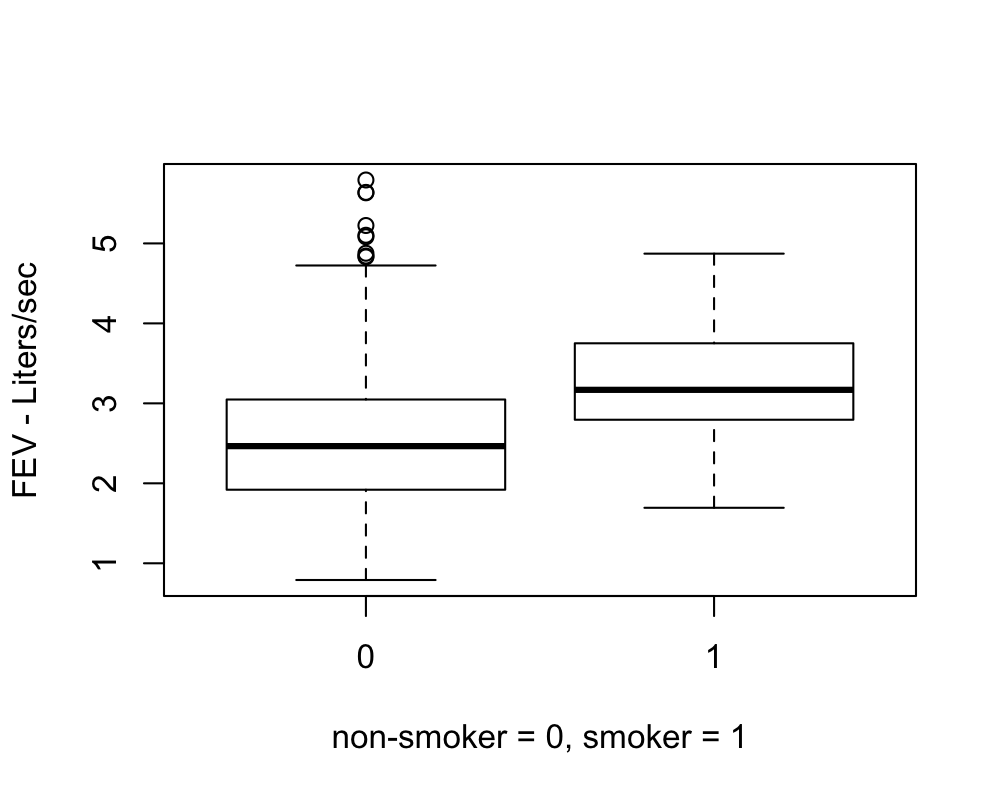
\includegraphics[width=\textwidth]{Figure}
  \caption{Box-and whisker plot comparing the FEV values of smokers and nonsmokers}
\end{figure*}

\item The slope is 0.711 and the intercept is 2.566 from the linear regression analysis. The intercept is just an average FEV value (L/s) for nonsmokers. The slope suggests that, on average, smokers have a higher FEV value of around 0.711 liters/second when compared to the FEV values of non-smokers.

\item The table below (Table 1) lists the slopes and intercepts of each strata-specific linear regression line.

\begin{table}[!ht]
\centering

\begin{tabular}{rlrr}
  \hline
 & Age & Intercept & Slope \\ 
  \hline
& 0-9 & 2.03 & -0.08 \\ 
& 10-11 & 2.85 & 0.25 \\ 
& 12-13 & 3.35 & -0.07 \\ 
& 14 and above & 3.85 & -0.45 \\ 
   \hline
\end{tabular}
\caption{Strata-specific slopes and intercepts of the effect of smoking on FEV values}
\end{table}

\item

The slopes are highly variable from one another. The slope from part (a) is 0.711, whereas all but one of the groups are negative. It makes sense that the slope is negative, as one would predict that non-smokers would have higher FEV values.
\\[10 pt]
As children grow, their FEV values should increase. The reason why it seems like smokers have better FEV values is because most smokers start their habit after the age of 14. There are very few smokers in the 0-9 category (1 smoker and 308 nonsmokers). In this data, there is aliasing between age and non-smoker on their effect of FEV.
\end{enumerate}
 
\section{LAD Regression}
\begin{enumerate}
\item Least Absolution Deviation (LAD) regression relies on the idea of minimizing this quantity:
\begin{equation}
\sum_{i=1}^{n}\mid Y_{i} - a - bX_{i} \mid
\end{equation}
Here $\mid Y_{i} - a - bX_{i} \mid$ depicts absolute deviations. The median is also a value that minimizes absolute deviations.

LAD regression is not as easily interpretable as linear regression  but is not as sensitive to extreme values.\footnote{\label{1}LAD often produces non-unique solutions and analysis on the same dataset can result in varying slopes and intercepts}

\item The tables below show strata-specific LAD values and compare LAD with linear regression.

\begin{table}[ht]
\centering
\begin{tabular}{rlrr}
  \hline
 & age & intercept & slope \\ 
  \hline
& 0-9 & 1.99 & -0.0034 \\ 
& 10-11 & 2.81 & 0.29 \\ 
& 12-13 & 3.15 & 0.039 \\ 
& 14 and above & 3.73 & -0.33 \\ 
   \hline
\end{tabular}
\caption{Strata-specific slopes and intercepts of the effect of smoking on FEV values using LAD regression}
\end{table}

\begin{table}[ht]
\centering
\begin{tabular}{rlrr}
  \hline
 & age & lm & LAD \\ 
  \hline
& 0-9 & -0.08 & -0.00 \\ 
& 10-11 & 0.25 & 0.29 \\ 
& 12-13 & -0.07 & 0.04 \\ 
& 14 and above & -0.45 & -0.33 \\ 
   \hline
\end{tabular}
\caption{Slopes and intercepts of LAD and Linear Regression}
\end{table}

'lm' produces more extreme slopes for the '0 to 9', '12 - 13' and '14 and above' age groups.'lm' is more sensitive to extreme data points. For example, the 1 smoker in the '0-9' age group could have a big effect since the mean of smokers in that age group is just that one smoker. The same idea arises for the '12-13' age group. For the 14 and above age group, the range of FEV values are from 2.198 to 3.6595, this large spread could result in more extreme lm slope values.
\\[10 pt]
\end{enumerate}
\end{document}